% Shared preamble for the English summaries in this repository.
\documentclass[11pt,a4paper]{article}
\usepackage[margin=2.2cm]{geometry}
\usepackage[T1]{fontenc}
\usepackage[utf8]{inputenc}
\usepackage{lmodern}
\usepackage{amsmath,amssymb}
\usepackage{graphicx}
\usepackage{booktabs}
\usepackage{enumitem}
\usepackage[hidelinks]{hyperref}
\setlist{itemsep=2pt,topsep=4pt}
\setlength{\parindent}{0pt}
\setlength{\parskip}{5pt}
\graphicspath{{figures/}}
\newcommand{\summaryheader}[3]{%
  \begin{center}
    {\Large\bfseries #2}\\[3pt]
    {\large #1}\\[3pt]
    {\small Arshia Goshtasbi \textbullet{} MSc Electrical Engineering (Control), Iran University of Science and Technology \textbullet{} #3}
  \end{center}
  \vspace{2pt}\hrule\vspace{8pt}
  \noindent\textit{English summary of my original Persian report, which is kept as a PDF in this folder.}\par}

\begin{document}
\summaryheader{Multivariable Control, Take-home Exam}{Characteristic-locus Design for the AIRC and TGEN Models}{Autumn 1403 (2024)}

\section*{Task}
Carry out the characteristic-locus design procedure on two standard models from Maciejowski, \emph{Multivariable Feedback Design}:
\begin{itemize}
  \item AIRC, a $5$-state aircraft model with 3 inputs and 3 outputs (\texttt{Q1\_final.m});
  \item TGEN, a $6$-state turbo-generator model with 2 inputs and 2 outputs, designed for a lower bandwidth (\texttt{Q2\_final.m}).
\end{itemize}

\section*{Method}
The compensator is built in three frequency bands:
\begin{enumerate}
  \item \textbf{High frequency, $K_h$.} A real constant approximation of $G(j\omega_b)^{-1}$ by the ALIGN algorithm. From the SVD $G(j\omega_b)=U\Sigma V^*$, take $K_h=-\operatorname{Re}(UV^*)$, which reduces misalignment at the design frequency ($\omega_b=3$\,rad/s for AIRC, $0.5$\,rad/s for TGEN).
  \item \textbf{Medium frequency, $K_m$.} A lead compensator on each channel to improve phase margin.
  \item \textbf{Low frequency, $K_\ell$.} PI action on each channel for zero steady-state error.
\end{enumerate}
After each step I plotted the characteristic loci of $GK$, then the closed-loop step responses and the singular values of $S$ and $T$.

\section*{Re-running the code (R2023b)}
Both scripts run, and their plots are in \texttt{figures/}. However, the closed loop formed in each script, \texttt{CL = feedback(K\_total, eye(n))}, is \textbf{unstable}: its largest pole real part is $+0.34$ for AIRC and $+44.1$ for TGEN. The step-response plots diverge accordingly. Two things look like the cause:
\begin{itemize}
  \item the characteristic-loci check in the scripts only measures the distance to $-1$ and does not count encirclements;
  \item the sign of $K_h=-\operatorname{Re}(UV^*)$ may need to be the opposite.
\end{itemize}
I left the code as submitted rather than change it after the fact.
\begin{center}
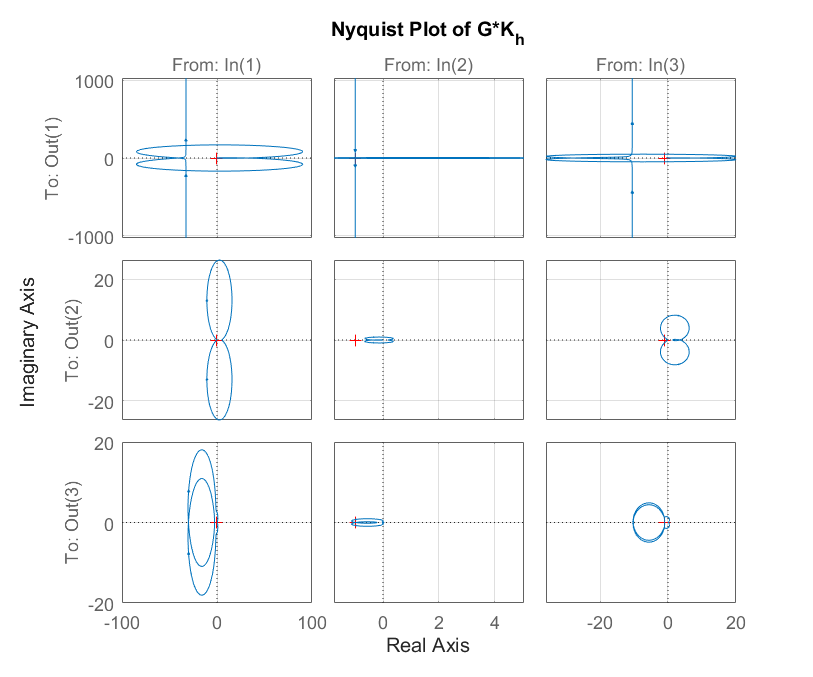
\includegraphics[width=0.48\linewidth]{Q1_final_1.png}\hfill
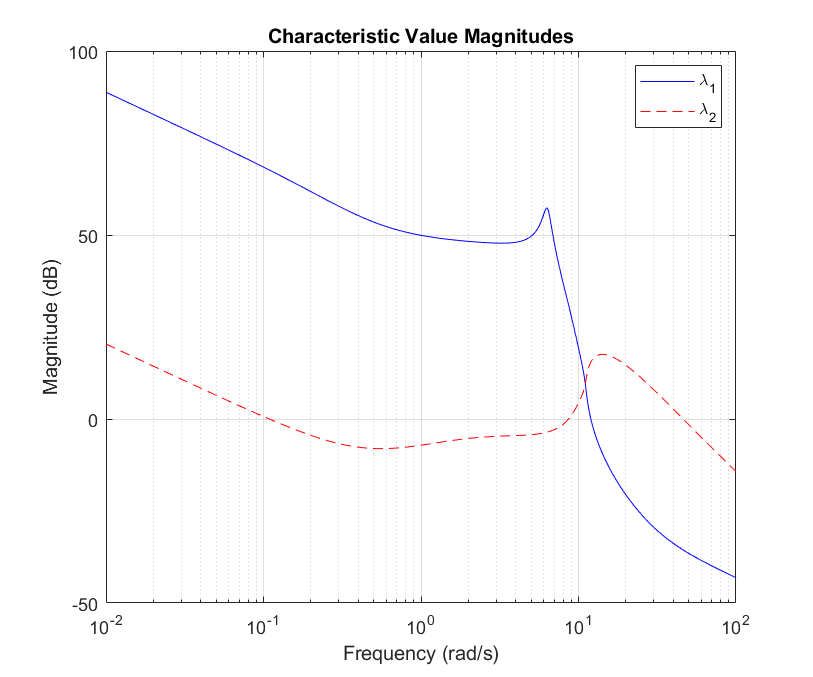
\includegraphics[width=0.48\linewidth]{Q2_final_6.png}\\[2pt]
{\small Left: characteristic loci of $GK_h$ for AIRC. Right: characteristic-value magnitudes for TGEN.}
\end{center}
\end{document}
